%% SECTION 2.3 %%
\section{Empirical Classification}
\label{subsec: empirical classification}

In reality, we do \emph{not} know the true distribution of $(X, Y)$. Instead, we are often working with finite sets of data $\mathcal{D}_n = \set{(X_1, Y_1), \dots, (X_n, Y_n)}$ (e.g., a training set), where the $(X_i, Y_i)$ are hypothetical future i.i.d.\ draws from $\P_{(X, Y)}$. Note that, if we build a classifier $h_n(X)$ based on this data, the classifier is random in two senses: it is a function of a random variable $X$, and it depends implicitly on the random data $\mathcal{D}_n$. Further, the expected error of $h_n$, i.e.,
\[
    L(h_n) = \Exp[\indSet{h_n(X) \neq Y}] = \P(h_n(X) \neq Y),
\]
is a \emph{random variable}, as it depends on the random data $\mathcal{D}_n$! Nevertheless, the excess risk
\[
    R(h_n) = L(h_n) - L^* \geq 0
\]
is always non-negative (in a deterministic sense, \emph{not} only almost surely). One approach of building a classifier based on the observed data $\mathcal{D}_n$ is the following: based on the observations $(X_1, Y_1), \dots, (X_n, Y_n)$, we estimate $\eta$ by $\eta_n$ and then construct the plug-in classifier $h_n = \indSet{\eta_n > \nicefrac{1}{2}}$. However, the (true) excess risk of $h_n$ is \emph{not} computable based on the sampled data alone and we cannot use any results for upper bounds on the excess risk $R(h_n)$ discussed in Section \ref{subsec: plug-in decisions}. A naive attempt to solve this problem is the definition of \emph{empirical risk}, which simply replaces the expected error $\Exp[l(h(X), Y)]$ by its empirical counterpart:

\begin{definition}
The \emph{empirical risk} of a classifier $h \colon \mathcal{X} \to \mathcal{Y}$ is given by
\[
    \hat L_n(h) = \frac{1}{n} \sum_{i=1}^n l(h(X_i), Y_i).
\]
\end{definition}

The empirical risk $\hat L_n(h)$ of a classifier $h$ is an \emph{unbiased estimator} of the \say{true} risk $L(h)$, i.e.,
\begin{equation}
\label{eq: bias of empirical risk}
    \highlightMath{
        \Exp[\hat{L}_n(h)] = \frac{1}{n} \sum_{i=1}^n \Exp[l(h(X_i), Y_i)] = \frac{1}{n} \sum_{i=1}^n \Exp[l(h(X), Y)] = L(h),
    }
\end{equation}
since $(X_i, Y_i)$ are i.i.d.\ draws from the distribution of $(X, Y)$.

Minimizing the empirical risk over all classifiers is pointless since, for every hypothetical data set, we can always construct a classifier with \emph{no} empirical risk by just mimicking the sampled data and classifying arbitrarily otherwise, e.g., the classifier
\[
    h_n(x) = \begin{cases}
        Y_i, \quad & x = X_i \text{ for some } i = 1, \dots, n \\
        0, \quad & x \notin \set{X_1, \dots, X_n}
    \end{cases}
\]
satisfies $\hat{L}_n(h_n) = 0$. This phenomenon is called \say{overfitting}: the classifier perfectly predicts the training data but fails to generalize to previously unseen data. Thus, in order to derive meaningful results from empirical risk minimization, we have to restrict ourselves to classifiers in a certain subset $\mathcal{H}$ of all measurable functions $h \colon \mathcal{X} \to \mathcal{Y}$.

\begin{definition}
The \emph{empirical risk minimizer} over $\mathcal{H}$ is defined as
\[
    \hat{h}^{\text{erm}} \in \argmin_{h \in \mathcal{H}} \hat{L}_n(h).
\]
\end{definition}

As just said, for meaningful results, $\mathcal{H}$ should be much smaller than the set of all classifiers. On the other hand, $\mathcal{H}$ should not be \emph{too} small either, because we want the empirical risk of $\hat{h}^{\text{erm}}$ to be close to the Bayes error. Often, we will be satisfied with a classifier $\hat{h}$ that is reasonably close to the empirical risk minimizer $\hat{h}^{\text{erm}}$ in the sense that
\[
    \hat{L}_n(\hat{h}) \leq \hat{L}_n(\hat{h}^{\text{erm}}) + \varepsilon, \quad \text{for small } \varepsilon > 0.
\]
Given a family $\mathcal{H}$, let $\bar{h}$ be a classifier that minimizes the \emph{true} risk\footnote{While we cannot construct this classifier from observing finite samples, it does certainly exist nonetheless.}, i.e.,
\[
    \highlightMath{
        \bar{h} \in \argmin_{h\in \mathcal{H}} L(h).
    }
\]
Note that it is impossible to construct such a classifier -- often called an \emph{oracle} -- from data alone. Nevertheless, we can attempt to find a classifier $\hat{h}$ that mimics the performance of the oracle $\bar{h}$ in the sense that we can hope to prove a bound of the form
\begin{equation}
    \label{eq: oracle inequality}
    L(\hat{h}) \leq L(\bar{h}) + \text{something small}.
\end{equation}
Such inequalities are often called \emph{oracle inequalities} for the simple reason that they involve the oracle $\bar{h}$. In \eqref{eq: oracle inequality}, we once again see the trade-off regarding the size of $\mathcal{H}$. If $\mathcal{H}$ is small, the performance of the oracle $\bar{h}$ is likely to suffer, while it might be possible to approximate $\bar{h}$ quite closely. If, on the other hand, $\mathcal{H}$ is quite large, the oracle $\bar{h}$ will be very powerful, but approximating $\bar{h}$ becomes statistically more difficult.

Ultimately\footnote{Remember that $L(\hat{f)}$ is a random variable!}, we want to prove tail bounds or bounds in expectation of the form
\[
    \P(L(\hat{h}) \leq L(\bar{h}) + \Delta_{n, \delta}(\mathcal{H})) \geq 1 - \delta,
\]
where $\Delta_{n, \delta}(\mathcal{H})$ is a function of $\mathcal{H}$ depending on the sample size $n$ and the desired level of confidence $\delta$.

\begin{figure}
    \centering
    \begin{tikzpicture}
        \node[above right, inner sep=0] (image) at (0,0) {
            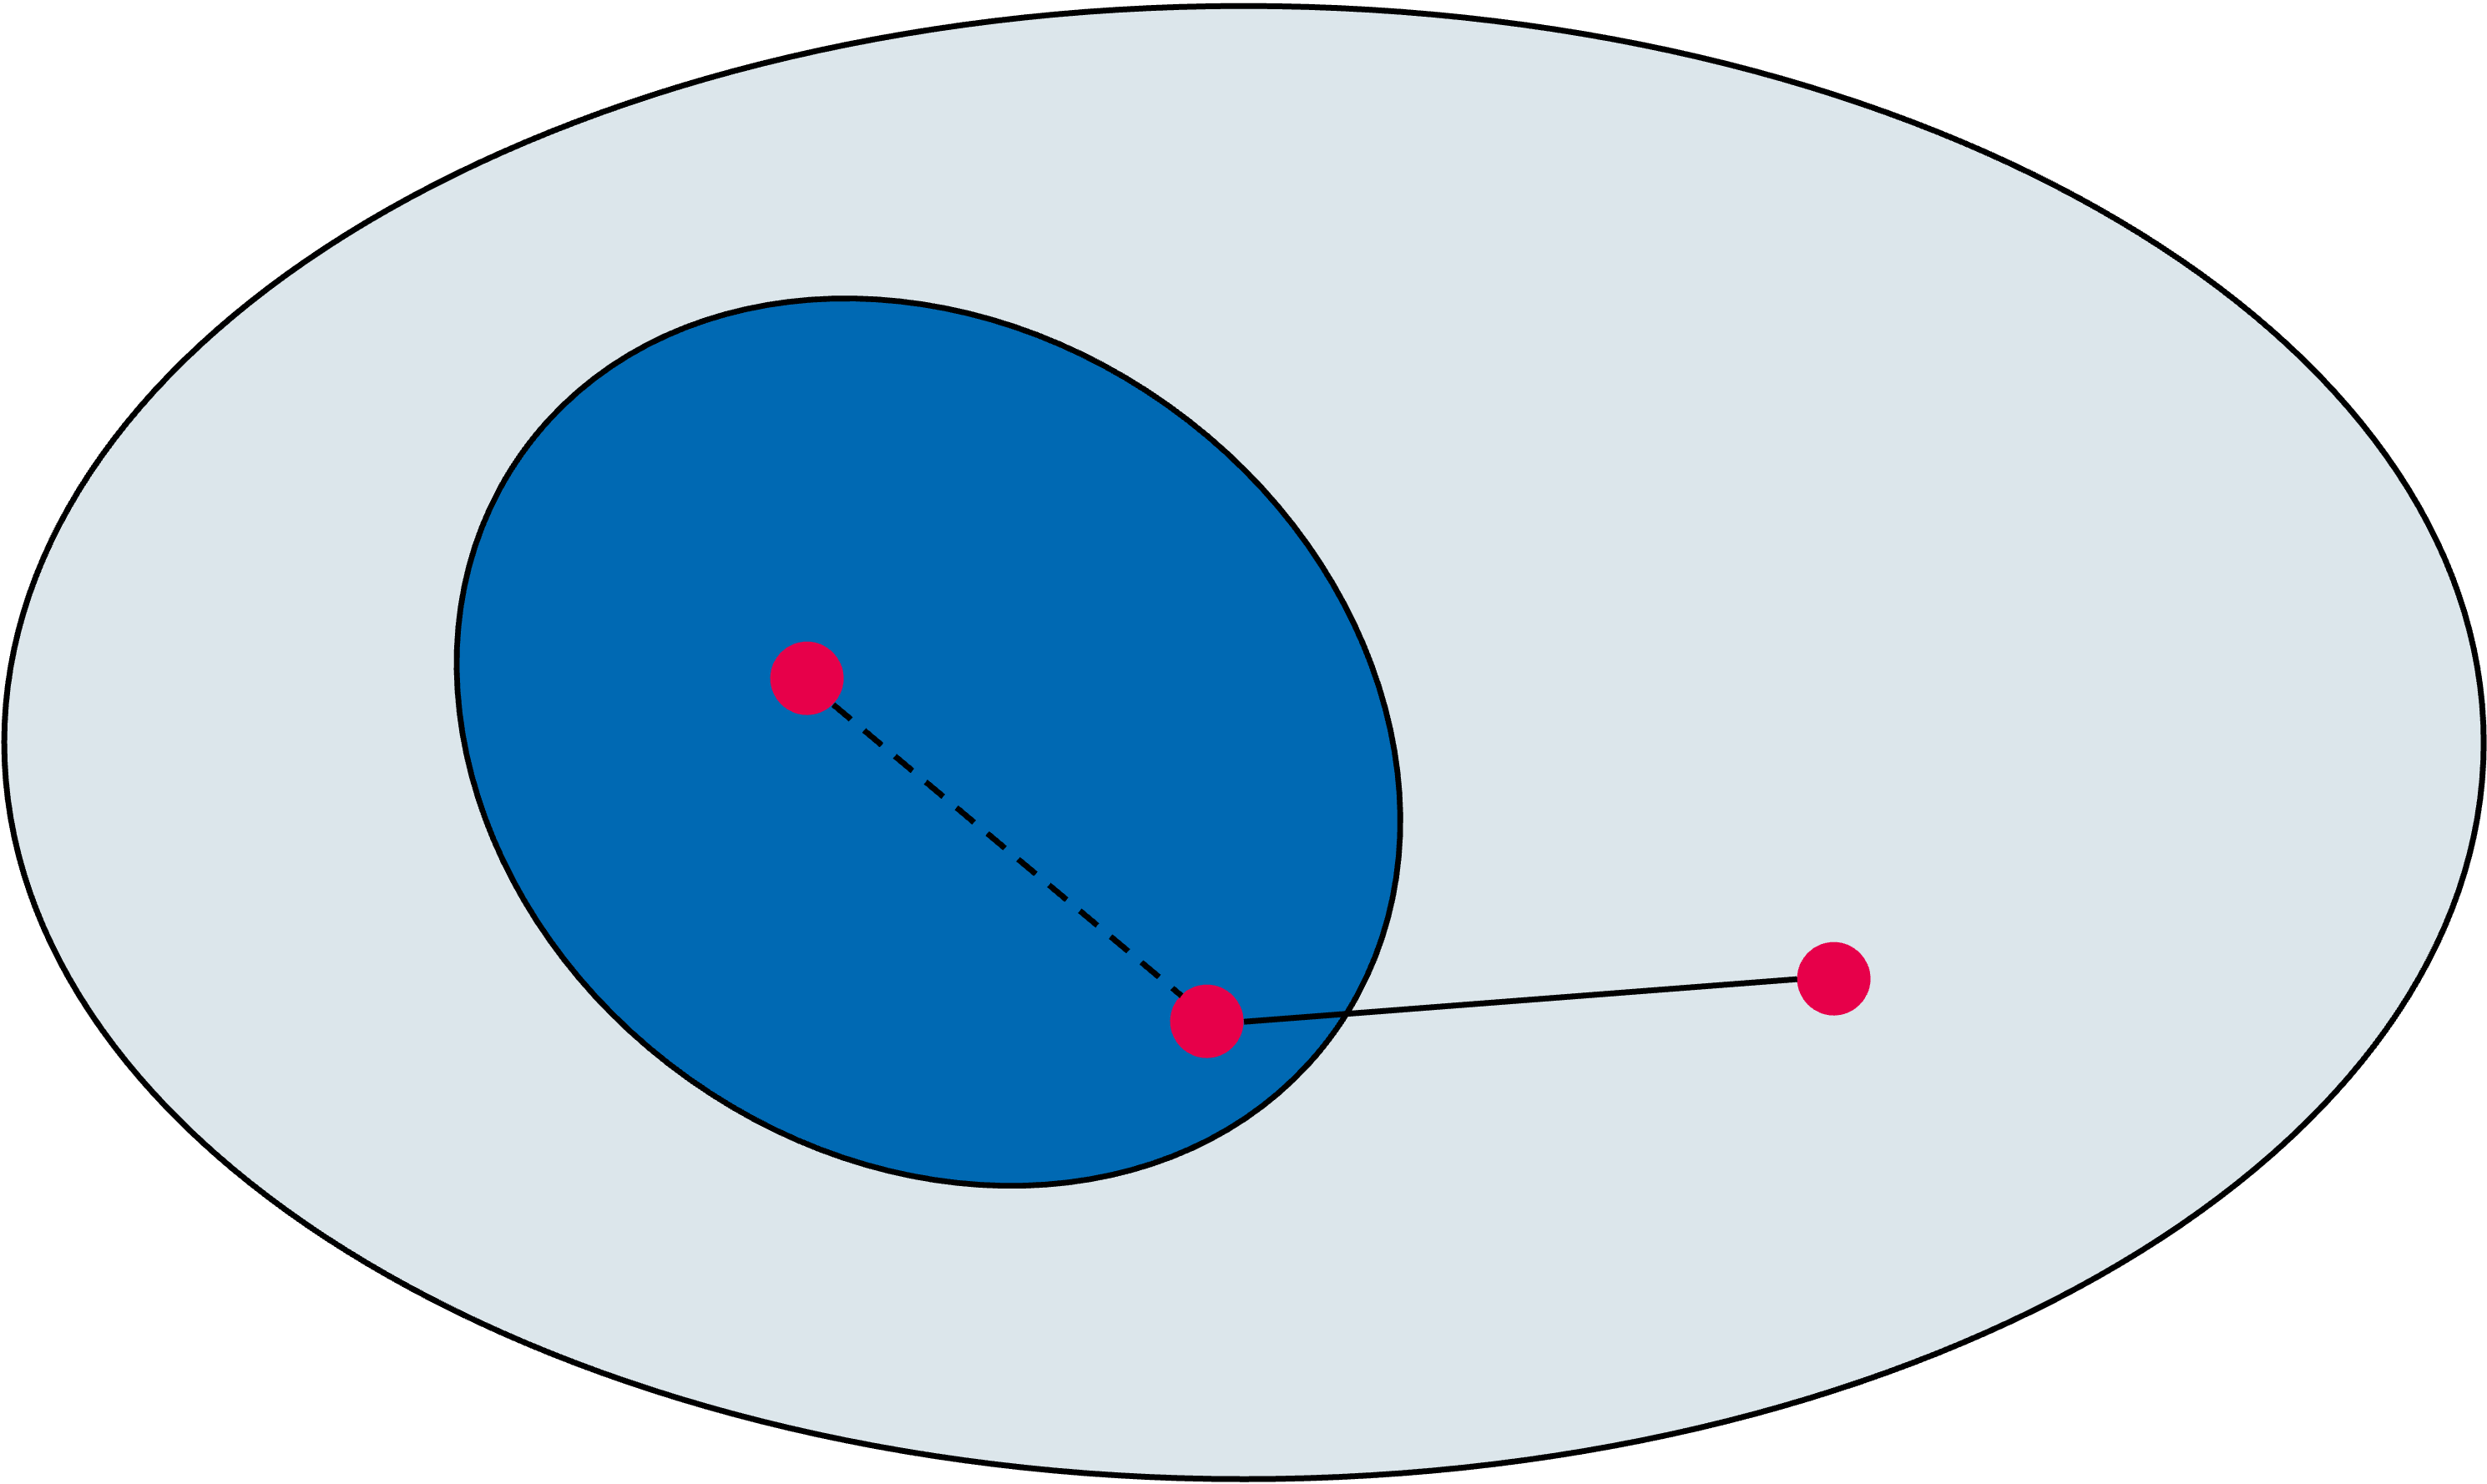
\includegraphics[width=0.5\textwidth]{other/estimation-approximation-error}
        };

        % Create scope with normalized axes
        \begin{scope}[
            x={(image.south east)},
            y={(image.north west)}]
         
            % Grid to properly align annotations
            % \draw[help lines, step=0.1] (image.south west) grid ($(image.north east) + (0.001,0)$);

            % Annotate image
            \node[] at (0.42,0.73) {${\color{white} \mathcal{H}}$};
            \node[] at (0.28,0.54) {${\color{white} \hat{h}}$};
            \node[] at (0.44,0.23) {${\color{white} \bar{h}}$};
            \node[] at (0.78,0.27) {$h^{*}$};
        \end{scope}
    \end{tikzpicture}
    \caption{%
        Decomposition of the excess risk $R(\hat{h})$ into estimation error (dashed line) and approximation error (solid line). The light blue area represents all measurable functions $h \colon \mathcal{X} \to \mathcal{Y}$ of which we consider a subset $\mathcal{H}$.
    }
    \label{fig: estimation vs approximation error}
\end{figure}

Finally, note that we can decompose the excess risk $R(\hat{h})$ of a classifier as follows:
\[
    \highlightMath{
        R(\hat{h}) = L(\hat{h}) - L^* = \underbrace{L(\hat{h}) - L(\bar{h})}_{\substack{\text{estimation} \\ \text{error}}} + \underbrace{L(\bar{h}) - L^*}_{\substack{\text{approximation} \\ \text{error}}}
    }
\]
The second term is the \emph{approximation error} that is unavoidable once we fix a family of classifiers $\mathcal{H}$. Oracle inequalities provide a method to bound the first term, the \emph{estimation error}.
